% Teorema Thales dengan TikZ - Gunanto (pakgun.gezytech.web.id)
% Kompilasi: pdflatex tikz-teorema-thales.tex
\documentclass[tikz]{standalone}
\usepackage{amsmath}
\usetikzlibrary{calc}
\definecolor{bg}{HTML}{171D2B}
\definecolor{acc}{HTML}{F7B538}
\definecolor{line}{HTML}{94A3B8}

\begin{document}

% ===== Gambar utama: lingkaran, diameter AB, titik C, jari-jari OC =====
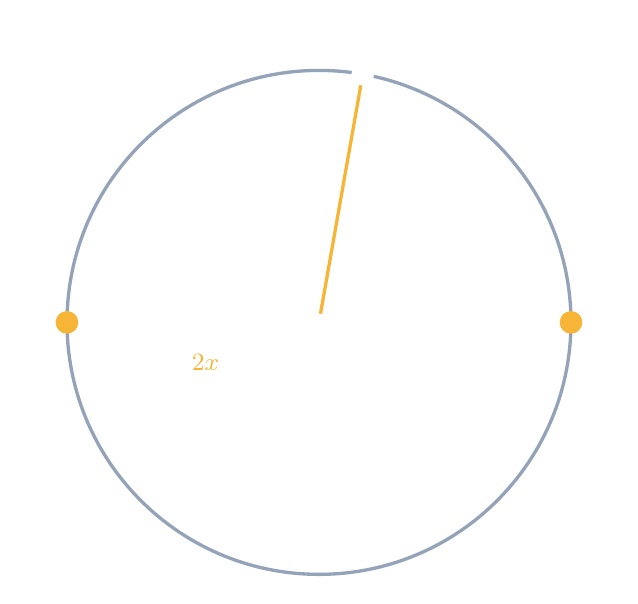
\begin{tikzpicture}[
  scale=3.2,
  every node/.style={color=white, font=\sffamily}
]
  % lingkaran
  \draw[line, very thick] (0,0) circle (1);
  % diameter AB
  \coordinate (A) at (-1,0);
  \coordinate (B) at (1,0);
  \coordinate (C) at (80:1);
  \coordinate (O) at (0,0);
  % jari-jari yang membentuk sudut pusat (warna aksen)
  \draw[acc, very thick] (A) -- (O) -- (B);
  \draw[acc, very thick] (O) -- (C);
  % sudut keliling: segitiga ABC (putih)
  \draw[white, very thick] (A) -- (C) -- (B) -- (A);
  % titik dan label
  \fill[acc] (A) circle (0.045) node[below left] {\textbf{A}};
  \fill[acc] (B) circle (0.045) node[below right] {\textbf{B}};
  \fill[white] (O) circle (0.035) node[below=3pt] {O};
  \fill[white] (C) circle (0.045) node[above=3pt] {C};
  % label sudut pusat dan sudut keliling
  \node[acc, font=\sffamily\small] at (-0.45,-0.16) {$2x$};
  \node[font=\sffamily\small] at ($(C)+(-0.16,-0.30)$) {$x$};
\end{tikzpicture}

% ===== Gambar kedua: dua posisi C, sudut ACB tetap 90 derajat =====
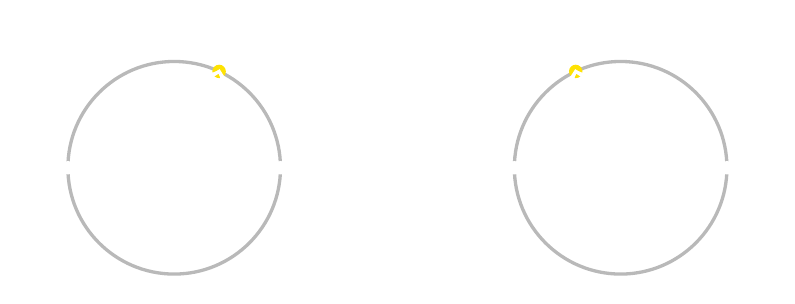
\begin{tikzpicture}[scale=1.35, every node/.style={color=white, font=\sffamily}]
  \foreach \x/\ang in {0/65, 4.2/115}{
    \begin{scope}[shift={(\x,0)}]
      \draw[gray!55, very thick] (0,0) circle (1);
      \fill[white] (-1,0) circle (1.8pt) node[below left=1pt] {A};
      \fill[white] (1,0) circle (1.8pt) node[below right=1pt] {B};
      \fill[yellow!85!orange] (\ang:1) circle (1.8pt) node[above=2pt] {C};
      \draw[white, very thick] (-1,0) -- (\ang:1) -- (1,0);
      % tanda siku-siku di C, mengikuti arah kedua tali
      \draw[white, thick] ([shift={(\ang+225:0.16)}]\ang:1)
        -- ++(\ang+45:0.16) -- ++(\ang+135:0.16);
    \end{scope}
  }
\end{tikzpicture}

\end{document}
